\documentclass[a4paper, 11pt]{article}
\usepackage[a4paper, total={6in, 8in}]{geometry}
\usepackage{graphicx}
\usepackage{subfigure}
\usepackage[colorlinks=true,linkcolor=black,anchorcolor=black,citecolor=black,filecolor=black,menucolor=black,runcolor=black,urlcolor=black]{hyperref}
\title{CS/SDP 262 Final Project Report}
\date{\today}
\author{Badvi, B.; Hamza, A.; Usaid, M.}

\begin{document}
\maketitle
\newpage
\tableofcontents
\newpage
\section {Introduction}
\subsection{Abstract}
Anthropocentrism and the capitalistic commodification of resources has led humans down a spiral of self-destruction, and equally increased a general disregard for nature. For most nature is an external entity, unbeknown to them that humanity is not exclusive from it. Following from this stems the negligence of intelligence shown in nature however, as we shall be exploring in our project, signs of intelligence can be found everywhere in nature. Our project deals with modelling the semi-intelligent behavior shown by an acellular organism known as Physarum Polycephalum or more commonly as Yellow slime mold. This organism has baffled biologist and researcher over its exhibition of intelligence besides the fact that it does not have a central nervous system. Surely without a central processing unit how can an organism function let alone solve difficult problems? Intriguingly enough P.Polycephalum cannot only perform basic life function but is able to solve many complex problems such as path optimization (Nakagaki et al., 2000). Research suggest that a pulsating flow of biochemicals within its tube-like structure handles P.Polycephalum’s intricate mobility and that the control of this fluid is the cause of its coordinated growth (Alim et al., 2013). Another research suggests that P.Polycephalum makes use of an external ‘spatial’ memory by using pheromones to mark visited regions (Reid et al., 2012).

\subsection{Purpose}
We are studying \textit{Physarum polycephalum} in the context of an agent-based model because it will allow us to better understand its situational behavior. By implementing an agent-based model we can think about the behavior of P. polycephalum in algorithmic terms. It will also allow us to introduce different parameters and observe the changes in the behavior based on those parameters. 

\subsection{Approach}

To try and obtain a holistic understanding and to model the behavior of P. polychephalum with a reasonable degree of accuracy, we will be using two different agent based models - each with a separate goal. The first ABM attempts to model the behavior of the slime mold as it coalesces around food sources in a maze. The maze is generated randomly and slime mold nuclei are randomly distributed across the maze and then are linked. The ABM intends to model the primitive behavior that the mold exhibits - it moves closer and closer to the food source, while the nuclei away from the food source tend to die off. However in doing so, it effectively solves the maze. 

\section {Details of Simulation Model}
\subsection{Agent Based Model (Minimum Food Distance)}

\begin{enumerate}
    \item \textbf{Motivation}
    
    \item \textbf{Agents}\\
    Two different types of agents are used, both serve a different purpose. One of these are used to generate a random maze when setup-maze is triggered. The main agents used in this simulation are an abstract of P.Polycephalum’s nuclei, these agents would own an attribute which would store the euclidean distance to the closest food source.
    
    \item \textbf{Environment}\\
    The environment is a Geo-spacial environment where we can setup mazes/walls to show how P.Polycephalum is able to overcome such scenarios.
    
    \item \textbf{Learning}\\
    The agent's movement is such that in each step they either move randomly, remain static, or they move towards a neighbor which is closer to the food node. The movement of an agent towards their neighbor is motivated from the fact that the nuclei prioritizes movement towards the direction it's obtaining the greatest nutrition hence an assumption is made that the flow of nutrients from the neighbor closest to the food source would be greater.
    
    \item \textbf{Interactions}\\
    Each agent is connected with another agent via a link these links are thence contribute to the movement the agents make throughout the simulation as shall be discussed further on.
    
    \item \textbf{Time}\\
    In reality Slime mold grows at about a centimeter an hour so it’s ideal to have the time scale of one tick being equal to an hour. Anything less would be redundant. In our environment we've made it as such so that a step of $0.3$ is equivalent to a step of $1 cm$ in a real-world scenario.
    
    \item \textbf{Variables and Constants} 
    \begin{itemize}
        \item \textbf{Global Variables}:
    \begin{enumerate}
        \item \texttt{prob\_random} - Represents the probability that a nucleus would move randomly, lies within the range $0$ and $1$ and the default value is $0.6$
        \item \texttt{prob\_static} - Represents the probability that a nucleus would remain static, lies within the range $0$ and $1$ and the default value is $0.6$
        \item \texttt{prob-reproduce} - Represents the probability that a nucleus divides creating another,lies within the range $0$ and $1$ and the default value is $0.15$
        \item \texttt{num-agents} - Represents the number of initial nuclei in the model, lies in range $0$ to $6000$ default value is $1000$
        \item \texttt{avgfooddist} - Represents the average distance of a nucleus from a food source.
    \end{enumerate}
    
    \item \textbf{Local Variables}
    \begin{enumerate}
        \item \texttt{distfood} - The Euclidean distance from the nucleus to the food source.
        \item \texttt{midptx}, \texttt{midptx1}, \texttt{midptx2} - The x-coordinates of three midpoints of a link. 
        \item \texttt{midpty}, \texttt{midpty1}, \texttt{midpty2} - The y-coordinates of three midpoints of a link. 
    \end{enumerate}
    \end{itemize}
    \item \textbf{Processes}\\
    Following processes are involved whilst setting up the environment:
    \begin{itemize}
        \item \texttt{setup-maze, setup-start-finish, make-maze} (Details of these processes can be referred from BAM's maze generation model inspired from \url{http://ccl.northwestern.edu/netlogo/models/community/BAM20Maze20Generator2)}
        \item \texttt{kill} This process is used to kill the maze-making agents once the maze is constructed
        \item \texttt{}
        

    \end{itemize}
    
    \item \textbf{Stochastic Measures}
    
    \item \textbf{Actions}
    
    \item \textbf{Inputs} \\
    This ABM does not take any input. 
    \item \textbf{Outputs}
    
    \end{enumerate}
    
\newpage
\subsection{Agent Based Model (Minimum Spanning Network)}
    
\begin{enumerate}
    \item \textbf{Motivation}
    \item \textbf{Agents}
    \begin{itemize}
        \item Nuclei 
        \item Food 
    \end{itemize}
    \item \textbf{Environment}
    \item \textbf{Learning}
    \item \textbf{Interactions}
    \item \textbf{Time}
    
    \item \textbf{Variables and Constants}
    \item \textbf{Processes}
    \item \textbf{Stochastic Measures}
    \item \textbf{Actions}
    \item \textbf{Inputs}
    \begin{itemize}
        \item Number of Food Nodes
        \item Angle of Vision
        \item Number of Nuclei
        \item Nuclei Secretion
        \item Food Secretion
        \item Evaporation Rate
        \item Step
    \end{itemize}
    \item \textbf{Outputs}
    \end{enumerate}
\newpage

\section{Analysis of Data}
Since, the primary goal of this project was an inquiry into the inner workings of the slime mold, we chose to not limit our study to just using ABM's. Through the use of the ABM we built that is referenced in section 2.2 we were able to acquire 3 independent variables that could be used to model the slime mold, and predict its decisions. We did this by using the BehaviorSpace tool present in Netlogo 6.1. We set out a range of changes in the independent variables that we were interested in to see how these changes impact the final average euclidean distance from the two food sources. The experiment was setup as follows: 
\begin{center}
    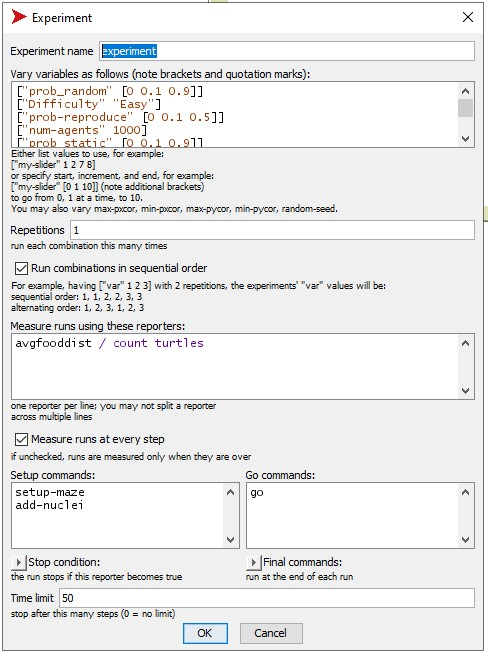
\includegraphics[scale=0.7]{Images/behaviorspace.jpg}
\end{center}
We were able the run the experiment twice and obtained 920 datapoints, which we then analysed using Python, and some libraries. Through this we were able to obtain visualization between the 3 independent variables and the dependent variable.
\begin{figure}[!h]
\centering
\subfigure[]{
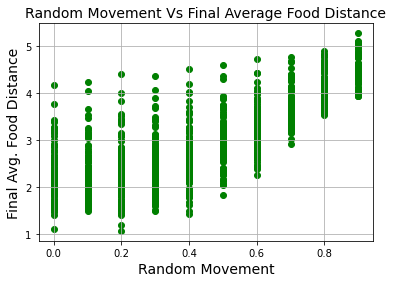
\includegraphics[width=0.43\textwidth]{Images/rndmove.png}
}
\subfigure[]{
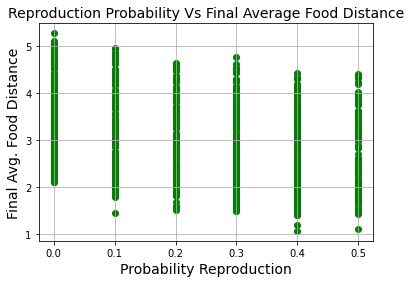
\includegraphics[width=0.45\textwidth]{Images/rndprod.png}
}

\subfigure[]{
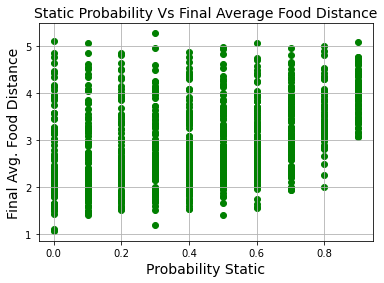
\includegraphics[width=0.5\textwidth]{Images/rndstatic.png}
}
\caption{Scatter Plots of 3 Independent Variables against the Dependent Variable}
\label{fig:whatever}
\end{figure}
\section{Limitations of the Model}
\subsection{Computational Limitations}
Since, our project was focused on an organism that has trillions of of nuclei, we knew computational complexity would be a problem for us from the start. We tried to explore avenues of incorporating multi-threading or perhaps use the CUDA cores of the discrete GPUs in our machines but that required the usage of another ABM modelling software called, Flame GPU. This was, obviously, outside the defined scope of the project so we were unable to rectify this issue.
\subsection{Linking the Nuclei}
Another major challenge was to ensure that links were being formed properly. We had to make sure that the links between two nuclei do not cross over a wall in the maze (a white patch). We simulated the slime's inability to create linkages through walls by simulating only links that were not crosses the wall. We calculated the 3 midpoints across each link and if any of those were intercepting the $x$ and $y$ coordinates of a white patch, we would eliminate the links. This added another layer layer of computational complexity within the model which furthered the limitations of the computational aspects of our ABM. 
\subsection{Preventing Clustering}
Another challenge was the fact that clusters form in areas in the maze. Theoretically, these clusters should die because they get stuck and cannot access food source, and are disconnected from the rest of the P. polycephalum. Unfortunately, eliminating these clusters would be very computationally expensive - which means that its more effective to let them be for the sake of practicality of the model, since the model itself is also computationally expensive due to the large number of nuclei and links that need to be iterated very often.  
\section{Conclusions}
\newpage
\section{Bibliography}

% \begin{enumerate}
%     \item Alim, K., Amselem, G., Peaudecerf, F., Brenner, M., & Pringle, A. (2013). Random network peristalsis in Physarum polycephalum organizes fluid flows across an individual. Proceedings of the National Academy of Sciences of the United States of America, 110(33), 13306-13311. Retrieved September 12, 2020, from \\ \url{http://www.jstor.org/stable/42712903}
%     \item Alim, K., Andrew, N., Pringle, A., Brenner, M. (2017). Mechanism of signal propagation in Physarum polycephalum. Proceedings of the National Academy of Sciences. Retrieved September 12, 2020, from \\\url{https://www.pnas.org/content/114/20/5136.short.}

%     \item Nakagaki, T., Yamada, H. & Tóth, Á. Maze-solving by an amoeboid organism. Nature 407, 470 (2000). \url{https://doi.org/10.1038/35035159}
    
%     \item Reid, C., Latty, T., Dussutour, A., & Beekman, M. (2012). Slime mold uses an externalized spatial "memory" to navigate in complex environments. Proceedings of the National Academy of Sciences of the United States of America, 109(43), 17490-17494. Retrieved September 12, 2020, from \url{http://www.jstor.org/stable/41829697}
    
%     \item Tero, A., Takagi, S., Saigusa, T., Ito, K., Bebber, D., Flicker, M., . . . Nakagaki, T. (2010). Rules for Biologically Inspired Adaptive Network Design. Science, 327(5964), new series, 439-442. Retrieved September 13, 2020, from \url{http://www.jstor.org/stable/40508592}
% \end{enumerate}

% Becker, Matthias (2011). [IEEE 2011 IEEE Congress on Evolutionary Computation (CEC) - New Orleans, LA, USA (2011.06.5-2011.06.8)] 2011 IEEE Congress of Evolutionary Computation (CEC) - Design of fault tolerant networks with agent-based simulation of Physarum polycephalum. 
\end{document}